% Copy to docs/ambiguities/lectureNN/main.tex when actual questions arise.
% Replace NN and the title; add real LNN-Qxx entries from the lecture ledger.
% Build from the repository root: make questions LECTURE=NN
% Store evidence crops in the new project's images/ folder.
% Questions are for later review. Do not stop transcription or ask live chat
% questions; deliver this PDF with the lecture, keeping unresolved items marked.
\documentclass[a4paper,12pt]{article}
\usepackage[margin=19mm]{geometry}
\usepackage{amsmath,amssymb,graphicx,xcolor}
\usepackage{fontspec}
\usepackage{xepersian}
\settextfont{XB Roya}
\setlatintextfont{Latin Modern Roman}
\definecolor{ink}{HTML}{173D75}
\graphicspath{{images/}}
\setlength{\parindent}{0pt}
\setlength{\parskip}{5pt}
\linespread{1.12}
\newcommand{\qtitle}[2]{{\Large\bfseries\color{ink} پرسش \lr{#1}: #2}\par}
\newcommand{\answer}{\medskip\textbf{پاسخ یا صورت مورد تأیید و تاریخ:}\par\vspace{18mm}\hrule\medskip}
\begin{document}
{\LARGE\bfseries پرسش‌های ابهام جلسهٔ ۱۷}\par
{\large مدول‌های تصویری و انژکتیو، جزوهٔ جبر پیشرفتهٔ دکتر خسروی}\par
شمارهٔ صفحه‌ها، شمارهٔ یک‌مبنای صفحه در فایل پی‌دی‌اف است.
ثبت در ۲۵ اکتبر ۲۰۲۶؛ پرسش برای بازبینی بعدی است و مانع پایان رونویسی نیست.
\begin{LTR}\small\texttt{sources/lectures/17 Injective and Projective Modules.pdf}\end{LTR}
\medskip\hrule\medskip
\qtitle{L17-Q01}{آرگومانِ نگاشت گسترش‌یافته در اثبات محک بئر}
\textbf{وضعیت:} باز؛ خوانش اسلایدها موقت است. پاسخی ثبت نشده است.\par
\textbf{نشانی منبع:} نسخهٔ \lr{primary}، صفحهٔ ۱۰، نیمهٔ پایین، فرمول تعریف
$\overline h$؛ شاهد مقایسه: صفحهٔ ۱۱، سه سطر نخستِ اثبات خوش‌تعریفی.
\textbf{عبارت منبع:} در صفحهٔ ۱۰، پس از تعریف
$\widetilde\theta:R\to J$، آمده است
\[
\overline h(m'+rn)=\widetilde h(m')+\widetilde\theta(rn).
\]
\begin{center}
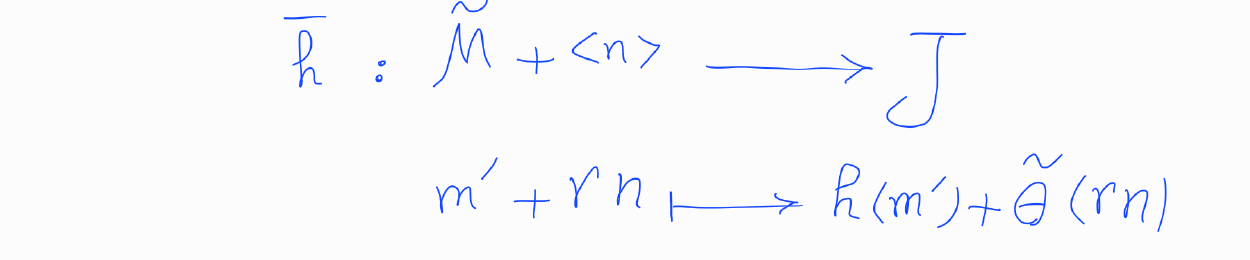
\includegraphics[width=.94\linewidth]{p10-extension.png}\\[-1pt]
{\small صفحهٔ ۱۰، تعریف نگاشت با دامنهٔ بزرگ‌تر}\\[3pt]
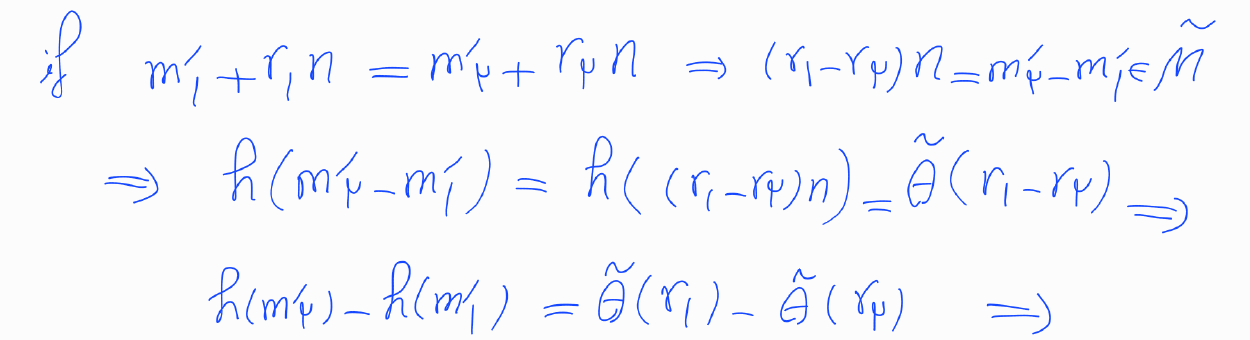
\includegraphics[width=.94\linewidth]{p11-scalar-arguments.png}\\[-1pt]
{\small صفحهٔ ۱۱، استفاده از آرگومان‌های اسکالر}
\end{center}
\textbf{خوانش‌ها و پیامد:} نقلِ لفظی، $\widetilde\theta(rn)$ است؛ اما
$rn\in N$ و دامنهٔ $\widetilde\theta$ برابر $R$ است، پس این کاربرد در حالت
کلی تعریف نشده است. خوانش پیشنهادی، $\widetilde\theta(r)$ است.
صفحهٔ ۱۱ از $\widetilde\theta(r_1-r_2)$ و $\widetilde\theta(r_i)$ استفاده
می‌کند و از این خوانش پشتیبانی می‌کند.

\textbf{پرسش برای بازبینی:} آیا در فرمول صفحهٔ ۱۰ باید
$\widetilde\theta(rn)$ به $\widetilde\theta(r)$ تغییر کند؟

\textbf{تصمیم موقت:} فرمول با $r$ و سه اسلاید پایانیِ برهان وابسته به آن،
با شناسهٔ همین پرسش موقت علامت خورده‌اند؛ اصلاح قطعی به منبع نسبت داده نشده است.
\par
\answer
\newpage
\qtitle{L17-Q02}{عدد حلقه در مثالِ مدول تصویریِ ناآزاد}
\textbf{وضعیت:} باز؛ عدد $6$ در اسلایدها خوانش موقت است. پاسخی ثبت نشده است.\par
\textbf{نشانی منبع:} همان فایل و نسخهٔ \lr{primary}، صفحهٔ ۵، مثالِ پایین
صفحه، زیرنویس‌های حلقه و مخرجِ یادداشت قرمز؛ دو نتیجهٔ بلافاصله پس از آن
در بالای صفحهٔ ۶ آمده‌اند.
\begin{LTR}\small\texttt{sources/lectures/17 Injective and Projective Modules.pdf}\end{LTR}
\textbf{عبارت منبع:} تجزیهٔ $\mathbb Z_{?}\cong\mathbb Z_2\oplus\mathbb Z_3$
و یادداشت قرمزِ $\mathbb Z_{?}=\mathbb Z/(?\mathbb Z)$، با ادعای
تصویری‌بودن و ناآزادبودنِ دو جمعوند.
\begin{center}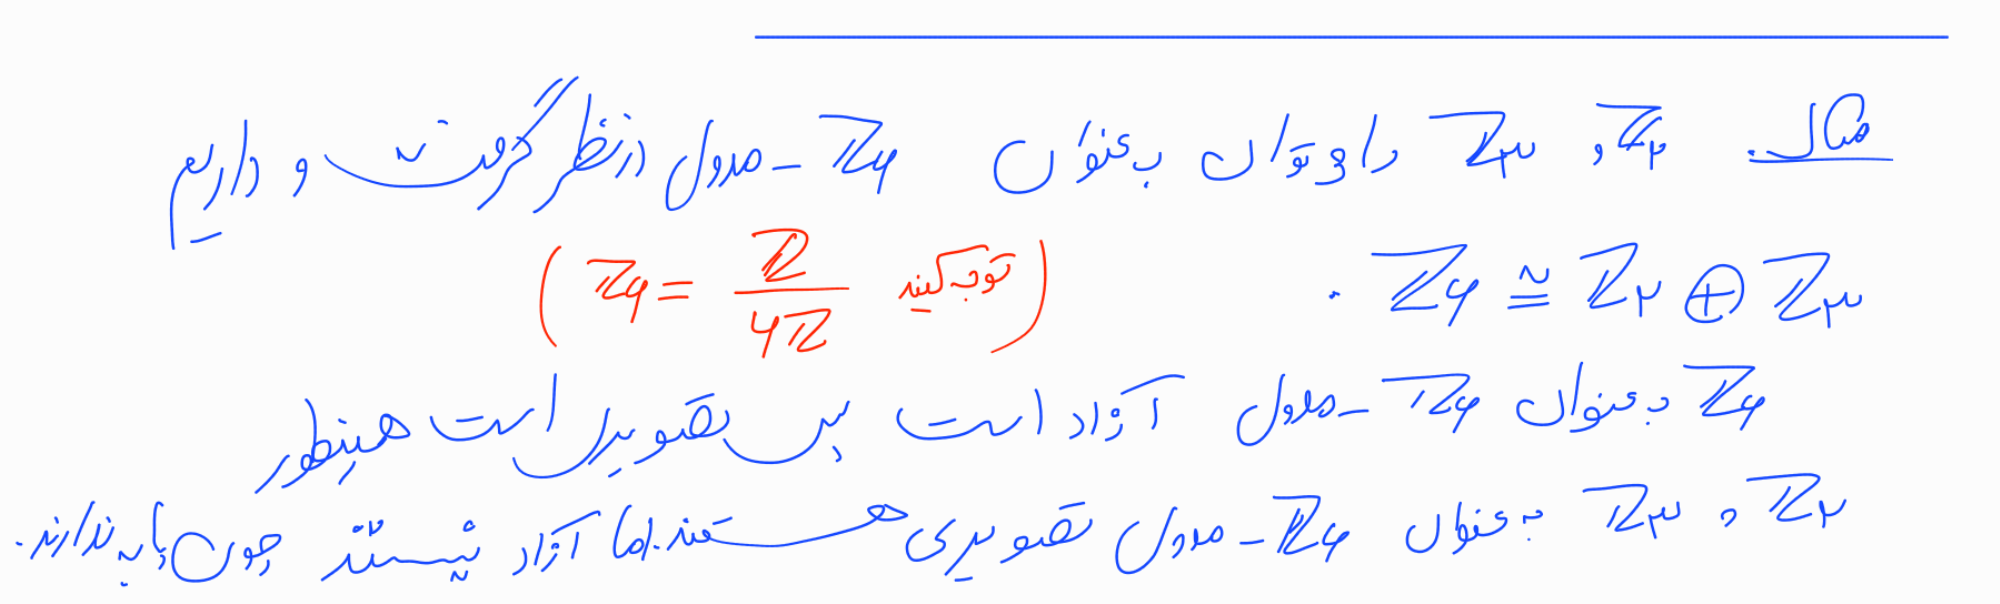
\includegraphics[width=\linewidth]{p05-cyclic-ring.png}\end{center}
\textbf{خوانش‌های ممکن:} عددِ $6$ با تجزیه سازگار است؛ اما شکل زیرنویس آبی
به $9$ و شکل عددِ مخرج قرمز به $4$ نیز شبیه است. بزرگ‌نمایی به تنهایی
خوانشِ لفظیِ مطمئنی نمی‌دهد. این شباهت‌ها خوانش قطعیِ $4$ یا $9$ نیز نیستند.

\textbf{دلیل پرسش:} سمت راستِ تجزیه $6$ عضو دارد. اگر عدد سمت چپ $4$ یا
$9$ باشد، این تجزیه نمی‌تواند درست باشد و ساختار مدولیِ مثال نیز باید دوباره
مشخص شود. سازگاریِ ریاضی، به تنهایی تأییدِ قطعیِ رقم دست‌نویس نیست.

\textbf{پرسش برای بازبینی:} آیا همهٔ زیرنویس‌های حلقه و مخرجِ یادداشت قرمز
در این مثال $6$ هستند؟ اگر عدد دیگری منظور است، صورت مورد نظرِ تجزیه و
حلقهٔ اسکالر کدام است؟

\textbf{تصمیم موقت:} مثال با حلقهٔ $\mathbb Z_6$ نقل شده و آشکارا موقت است.
اسلایدِ دو نتیجهٔ صفحهٔ ۶ نیز موقت‌بودنِ شاهدِ مثال را یادآوری می‌کند.
این پرسش، نتیجهٔ قطعی یا اصلاحِ تأییدشده‌ای به منبع نسبت نمی‌دهد.
\par\answer
\end{document}
